%\documentclass{acm_proc_article-sp}
\documentclass{sig-alternate}
\usepackage{latexsym,amssymb,amsmath}
\usepackage{epic,eepic}
\usepackage{graphicx}
\usepackage{xspace}
\usepackage{url}
%\usepackage{hyperref}
%\usepackage{breakurl}
\setlength{\columnsep}{0.7cm}
\usepackage{macro,luca}
\usepackage{times}

\begin{comment}
\hypersetup{
%    bookmarks=true,         % show bookmarks bar?
%    unicode=false,          % non-Latin characters in Acrobat's bookmarks
%    pdftoolbar=true,        % show Acrobat's toolbar?
%    pdfmenubar=true,        % show Acrobat's menu?
    pdffitwindow=true,      % page fit to window when opened
    pdftitle={Measuring Author Contributions to the Wikipedia},    % title
    pdfauthor={B. Thomas Adler, Luca de Alfaro, Ian Pye, Vishwanath Raman},     % author
    pdfsubject={Wikipedia Contributions},   % subject of the document
    pdfnewwindow=true,      % links in new window
%    pdfkeywords={keywords}, % list of keywords
    colorlinks=false,       % false: boxed links; true: colored links
    linkcolor=black,          % color of internal links
    citecolor=black,        % color of links to bibliography
    filecolor=black,      % color of file links
    urlcolor=blue,           % color of external links
    breaklinks=true
}
\end{comment}

\conferenceinfo{WikiSym '08,}{September 8--10, Porto, Portugal.}
\CopyrightYear{2008}
\crdata{978-1-60558-128-3/08/09}

\begin{document}
\sloppy

\newif
  \iflong
  \longfalse
\newif
  \ifshort
  \shorttrue

\pagestyle{plain}

\title{Measuring Author Contributions to the Wikipedia\titlenote{This 
    research has been
    partially supported by the CITRIS: Center for Information
    Technology Research in the Interest of Society.\\
    Copyright ACM, 2008.  This is the authors' version of the work.
    It is posted here by permission of the ACM for your personal use.
    Not for redistribution.  The definitive version was published in 
    Proceedings of WikiSym 2008.
    \vspace*{-5mm}
  }}

\numberofauthors{4}
\author{
B. Thomas Adler$^1$ \qquad
Luca de Alfaro$^2$ \qquad
Ian Pye$^1$ \qquad
Vishwanath Raman$^1$
\and
\alignauthor
	\affaddr{$^1$Computer Science Dept.} \\
	\affaddr{UC Santa Cruz, CA, USA} \\
	\email{\{thumper, vishwa, ipye\}@soe.ucsc.edu}
\alignauthor
	\affaddr{$^2$Computer Engineering Dept.} \\
	\affaddr{UC Santa Cruz, CA, USA} \\
	\email{luca@soe.ucsc.edu}
}

\maketitle

\begin{abstract}
\begin{abstract}
The Wikipedia is an experiment in group collaboration to
build an encyclopedia in an open way.
Perennial criticism centers around the lack of accountability
for authors, and the potential for misinformation.
The large community around the Wikipedia project actively
fixes errors as they are discovered, but an unending
stream of vandals and spammers chip
away at the good will of volunteers who
maintain the project for the collective good.
We suggest that an author reputation system and
an article text trust system can be used to focus
the volunteer effort on edits more likely to be a problem,
making more efficient use of the project's human resources.

In order to minimize the human effort diverted towards a reputation system,
we choose to preserve the current user experience as much as
possible.
To that end, we propose \textit{content-driven} reputation:
using only the version history, the content evolution of an
article is used to measure how well the authors
contribute to the Wikipedia.
When authors make contributions that are preserved over many
revisions, their reputation goes up.
We desire that author reputation be correlated with the
stability of the text they contribute ---
low reputation should be a predictor of author
contributions which will be edited or deleted.

Author reputation and article history are used as
inputs to our content-driven trust system.
Trust is computed on a per-word basis, with the
goal of highlighting changing portions of article text.
We desire that low trust correlate with text that
is deleted on the next revision, but we also don't want
to habituate users to our flagging.
These goals are somewhat contradictory, so we describe
how to measure and combine them.

We propose automated methods for evaluating the quality of
authors, and (separately) the text they create.
By relying on the history of edits, we can draw inferences about
the quality of the text that has come earlier in the history.
Instead of measuring ``truth,'' our reputation ideas
measure the ``group consensus'' in a piece of text.
As the article text stabilizes over time, we conclude that
it has reached a form which most members of the community can
reasonably agree on.
As group collaboration increases in prominence on the Internet,
we feel that this research will open the door on new applications
and quality measures.

\end{abstract}

\end{abstract}

% A category with the (minimum) three required fields
\category{H.5.3}{Information Interfaces and Presentation}{Group
and Organization Interfaces}[Computer-supported cooperative work, 
Web-based interaction]
\category{K.4.3}{Computers and Society}{Organizational Impacts}
[Computer-supported collaborative work]
%A category including the fourth, optional field follows...
\category{J.4}{Social and Behavioral Sciences}{Miscellaneous}

\pagebreak

\section{Introduction}

History is filled with examples of partnerships, people collaborating
to create something larger than they could achieve on their own;
but how do you value the contributions of the individuals?
How do we say whether Apple benefited more from the technical
designs of Steve Wozniak or the design intuition of Steve Jobs?
The reality is that the very notion of what is a \intro{contribution}
depends on perspective and relative priorities of importance.
When multiple authors work on a single book, how do you measure
who did the work, and how should the revenue be split?

Today, online collaboration is growing by leaps and bounds,
fostered under the name \intro{Web~2.0}: ``the actvities of
users generating content (in the form of ideas, text,
videos, or pictures) could be \textit{harnessed} to
create value''~\cite{wiki:Web20}.
In Silicon Valley, we hear examples every day of companies
built atop the contributions of their users:
Google, Facebook, Twitter, Flickr, to name a few famous ones.
For the most part, these sites operate under a motto
of ``more is better,'' and only a few sites try to estimate
a quality of contributions (\eg Amazon and eBay).
These sites are distinct from the Wikipedia, because although
users generate content, and even collaborate in some sense,
they don't actually work on the same content.

Within the Wikipedia community, there has been some discussion
about measuring contritbutions~\cite{Wales2005,Swartz2006},
in the context of whether some restrictions would improve
the overall quality of the Wikipedia.
Another motivation for understanding contributions by
users is for attribution purposes: the Creative Commons license
that the Wikipedia content is available under requires attribution
of all authors, which is currently taken to include spammers
and other vandals.
When wikis~\cite{Leuf2001} are used in a corporate setting,
measuring contributions can be a proxy for the productivity
of workers.

In this chapter, we examine multiple ways that contributions
can be defined within the Wikipedia.
We explore the distribution of users under these different measures,
and make some observations.


\section{Definitions}

The following notation will be used throughout the paper.
We consider the set $\pages$ of all articles in the main English 
Wikipedia.
We denote the set of authors of pages on the Wikipedia by
$\authors$.
We assume that we have $n > 0$ versions $v_0, v_1, v_2,
\ldots, v_n$ of a page $p$; version $v_0$ is empty, and version 
$v_i$, for $1 \le i \le n$, is obtained by an author performing 
a revision $r_i : v_{i-1} \leadsto v_i$.
Since each revision $r_i$ is performed by one author, we refer
to the author who edited revision $r_i$ as $a_i$.
We denote the set of all revisions of a page by $\revisions$.
We refer to the change set corresponding to 
$r_i : v_{i-1} \leadsto v_i$ as the edit performed at $r_i$ : the 
edit consists of the text insertions, deletions, displacements, 
and replacements that led from $v_{i-1}$ to $v_i$. 
We define the map $E : \authors \times \pages \to 2^\revisions$, 
which given an author $a \in \authors$ and a page $p \in \pages$, returns a
set of revisions that were created by author $a$ for page $p$.
When editing a versioned document, authors commonly save several 
versions in a short time frame.
We filter the versions, keeping only the last of consecutive 
versions by the same author; we assume thus that for $1 \le i \le n$
we have $a_{i-1} \ne a_i$.
Every version $v_i$ for $0 \le i \le n$, consists of a sequence
$[w_1^i,\ldots,w_{m_i}^i]$ of words, where $m_i$ is the number
of words in $v_i$; version $v_0$ consists of the empty sequence.

\smallskip

\noindent\textbf{Quantity Measures.}

Given a series of versions $v_0,\ldots,v_n$ of a page $p$, we assume
that we can compute the following quantity measures:
%
\begin{itemize}

\item $txt(v_i, v_j)$, for $0 < i \le j \le n$, is the amount of
	text (measured in number of words) that is introduced by
	$r_i$ in $v_i$, and that is still present (and due to the same
	author $a_i$) in $v_j$.
	$txt(v_i,v_i)$ is the amount of new text added by $a_i$ through
	$r_i$.
	We define $txt(r_i) = txt(v_i,v_i)$, and refer to this
	as the \intro{text contribution} of $r_i$.

\item $d(v_i, v_j)$, for $0 \le i < j \le n$, is the
	\textit{edit distance} between $v_i$ and $v_j$,
	and measures how much change
	(word additions, deletions, replacements, displacements, etc.)
	there has been in going from $v_i$ to $v_j$.
	We define $d(r_i) = d(v_{i-1}, v_i)$, for the \intro{edit contribution}
	made in a revision $r_i$.
\end{itemize}
%
There are several ways to compute edit distance~\cite{Levenshtein66,TichyEditDist},
usually based on insertions and deletions of characters.
Our formulation is instead based on words as the fundamental unit,
to more closely approximate how people perceive edits.
We define the edit distance in terms of the following quantities:
$I(v_i, v_j)$ is the number of words that are inserted;
$D(v_i, v_j)$ is the number of words that are deleted;
$M(v_i, v_j)$ is the number of words that are moved, times the fraction
of the document that they move across \cite{Adler2007}.
The edit distance between two versions, $v_i$ and $v_j$, is
then given by:
%
\[
d(v_i, v_j) = \max(I, D) - \frac{1}{2}\min(I, D) + M
\]
%
A more precise treatment of this definition is available
in~\cite{Adler2007}, along with reasoning for this particular
choice of edit distance and a discussion of text tracking
for authorship.


\smallskip

\noindent\textbf{Quality Measures.}

In addition to the quantity measures defined above, we define the
following quality measures.
We first consider the edits in a revision $r_i$ made by author
$a_i$.
Given $d(v_{i-1}, v_i)$, the edit distance between versions
$v_{i-1}$ and $v_i$, we would like to associate a higher edit
quality to revision $r_i$ if the edits made take the page
closer to subsequent versions of the page.
For example, if none of the edits made in $r_i$ are reverted
in subsequent revisions, then the edits made in $r_i$
have taken the page in the same {\em direction\/} as subsequent 
versions of the page and hence merit the highest quality measure.
We define $\editquality(v_i, v_j)$, the quality of the edits
performed in revision $r_i$ of a page (with respect to $v_j$) as follows:
%
\[
\editquality(v_i, v_j) = 
\frac{d(v_{i-1}, v_j) - d(v_i, v_j)}{d(v_{i-1}, v_i)}
\]
%
The triangle inequality generally holds, so that
$\editquality(v_i, v_j)$ typically varies from
$-1$ for revisions which are completely reverted,
to $+1$ for revisions which are completely preserved;
when the value falls outside this range, we
cap it to one of these two values.

Due to the occasional vandalism that happens, we prefer to
judge quality using several succeeding versions.
We define a map $J : \revisions \to 2^\revisions$,
such that if $r_i$ is a revision of a page $p$, 
$J(r_i)$ consists of the first ten revisions after $r_i$ that have
author different from that of $r_i$.
If there are fewer than ten revisions after $r_i$ that have author
different from that of $r_i$, then $J(r_i)$ returns all such
revisions. 
We use the versions in $J(r_i)$ as judges of the quality of $r_i$.
We define the {\em average edit quality} $\avgeditquality(r_i)$
of a revision $r_i$ with $|J(r_i)| \neq \emptyset$ as follows:
%
\[
\avgeditquality(r_i) = 
\frac{1}{|J(r_i)|} \cdot \left( \sum_{r_j \in J(r_i)} 
  \editquality(v_i, v_j) \right)
\]
%
Thus, $\avgeditquality(r_i)$ is the average of the \editquality values
determined by each of the judges of $r_i$.

The quality of a text contribution to a page is a function of
how much of the original text was edited out in subsequent
revisions of the page.
If none of the text was removed, then the text quality of revision
$r_i$ should be $1$.
One model for how text behaves over time is that it decays in
an approximately geometric fashion:
the largest chunk that is deleted is right after text is added,
and subsequent revisions remove smaller and smaller chunks
until what is left is the stable core which is generally
accepted by other authors.
We define the text quality measure 
$\textquality(r_i)$ as the solution to the following equation that
expresses text decay in this manner:
%
\[
\sum_{r_j \in J(r_i)} txt(i,j) = 
txt(i,i) \cdot \left( 1 +\sum_{r_j \in J(r_i)} (\textquality(r_i))^{j-i} \right)
\]
%
The resulting value for $\textquality(r_i)$ ranges from $0$
for text which is completely removed, to $+1$ for text which
is completely preserved.

A different way to measure the quality of a text contribution
is to simply sum the amount of text that remains, over the
succeeding revisions.
For a revision $r_i$, by considering the amount of original text 
introduced in $r_i$ that survives in the next ten revisions, we 
define the following additional quality measure for text 
contributions,
%
\[
\textlongevity(r_i) = \frac{1}{txt(i,i)} \cdot
\left( \sum_{r_j \in J(r_i)} txt(i,j) \right)
\]
%
This value generally ranges from $0$ for text which is immediately removed,
to $+10$ for text which completely survives all ten revisions.
(Due to how text tracking works, if a piece of text is copied within
an article, the original author might receive credit for more
words than she originally wrote.)


\subsection{Contributions of this Work}

We propose research into two ideas that can be leveraged
into tools to assist well-intentioned users.
The first is a \intro{reputation system} for users, which measures
their contributions to the Wikipedia with respect to some
notion of the group consensus.
The second idea is a \intro{trust system} for text,
which models the amount of review each word receives from editors
to quantify the likelihood that the text will persist
into the future.
One of our goals is to preserve the current user experience,
as much as possible.


Our basic idea is to take advantage of the Wikipedia's version history
for articles to develop content-driven \intro{reputation systems}
and \intro{trust systems}~\cite{WikiMTWtrust06,McGuinness06,www07,WikiTrust2008}.
A content-driven reputation system is one which uses
the version history to measure the work performed by users;
users gain reputation when they make
contributions to the Wikipedia which are deemed valuable, and lose reputation
when they make contributions which are reverted.
A content-driven trust system uses the version history
to predict the quality of the text submitted, incorporating
information from the reputation system.
The trust system acts as a guide to users,
indicating recent edits that need more scrutiny.
The advantage of content-driven systems,
as opposed to manual rating systems, is that they do
not significantly alter the user experience.

We have implemented an initial prototype of our reputation and
trust algorithms~\cite{www07,WikiTrust2008}.
This system takes as input an XML dump of a Wikipedia project,
analyzes the evolution of articles to determine lasting
contributions by authors, and computes a reputation for
each author based on the size and age of their contributions.
At the same time, a trust value is computed for each word
based on the reputations of authors who edit
regions of text nearby.
Our evalutions for both algorithms are very encouraging:
low reputation authors predominantly have their contributions
reverted, and low trust text is much more likely to be
deleted on the next revision than high trust text.
Further details of the algorithms and evaluations
are discussed in Sections~\ref{sec-reputation}
and~\ref{sec-trust}.

The course of our continued investigation is to examine
other applications of reputation and trust systems in
the context of the Wikipedia:


\section{Implementation}

As part of our research into author reputation
and text trust~\cite{Adler2007,WikiTrust08}, we have
created a modular tool for processing XML dumps from
the Wikipedia.
It analyzes all the revisions of a page,
filtering down the revisions to remove consecutive edits
by the same author, and computing differences between
revisions to track the author of each word and measure
how the author might have rearranged the page.
These results can be passed to any of several
modules to do additional processing; we use the tool
to reduce the enormous collection of data down to
a much smaller \textit{statistics file}.
We process the statistics file with a second tool,
which we instrumented to calculate the various
contribution measures we have defined.

Our analysis is based on main namespace (\texttt{NS\_MAIN})
article revisions from
the Wikipedia dump of February~6, 2007,
which we process to create a reduced statistics file.
The statistics file contains information about every version,
including the amount of text added, the edit distance from
the previous version, and information about how the edit
persists for ten revisions into the future.
To ensure that each version we considered had revisions
after it, we consider only versions before October~1, 2006.
After further processing on the file,
we used R~\cite{R2007}, an open source statistics package,
to analyze the resulting data.

\textbf{Bots.}
During the course of our analysis, we found that
some authors were extraordinary outliers for multiple measures.
Some investigation into the most extreme cases revealed
that bots were making automated edits to the Wikipedia,
and that a few bots dwarfed manual labor in the edit based
measures $\editlong$ and $\editonly$.
We also found that there are bots that improve content,
and bots that vandalize it.
We chose to identify bots as those with a username which
ends in the string ``bot;''
While this does not include every bot (especially
the ones that vandalize), it is a useful first approximation.
We found $614$ bots in total as of October~1, 2006.

\textbf{Vandals.}
There is a similar problem in trying to define vandals,
since such authors don't register themselves as such.
For our purposes, we decided to define a vandal
as someone who, on average, makes an edit which is
completely reverted.
Precisely, we define a vandal who meets one of two criteria:
$\quality{decay}{10}{} < 0.05$, or $\quality{elong}{10}{} < -0.9$.
We justify this choice in the next section.


\section{Analysis}

We begin our analysis with some information about the data
we are analyzing.
Our reduced statistics file includes over 25 million revision
records.
Figures~\ref{fig-revs-quality} and~\ref{fig-revs-contrib} were
created by drawing a random sample of 5 million records,
due to memory limitations of the software package.
%% CUT: Luca & Bo discussed this, and decided that it
%% would be distracting to the audience.  Since we're
%% already sampling 20%, most people won't take issue.
% ; three different samples of 5 million
% records produced nearly identical results.

In Figure~\ref{fig-revs-quality}, we show the frequency distribution
of the two quality measures
\quality{tdecay}{10}{} and \quality{elong}{10}{} over the revisions we sampled.
We see both measures are heavily biased towards $+1$, indicating that
most revisions to the Wikipedia are generally considered useful
by succeeding authors.
This confirms the intuition that more ``good people'' than
``bad people'' must contribute, otherwise the Wikipedia would
have a difficult time maintaining the community which
continues to extend the online encyclopedia in a useful way.
%
\begin{figure}[tbhp]
    \begin{center}
    \fbox{
    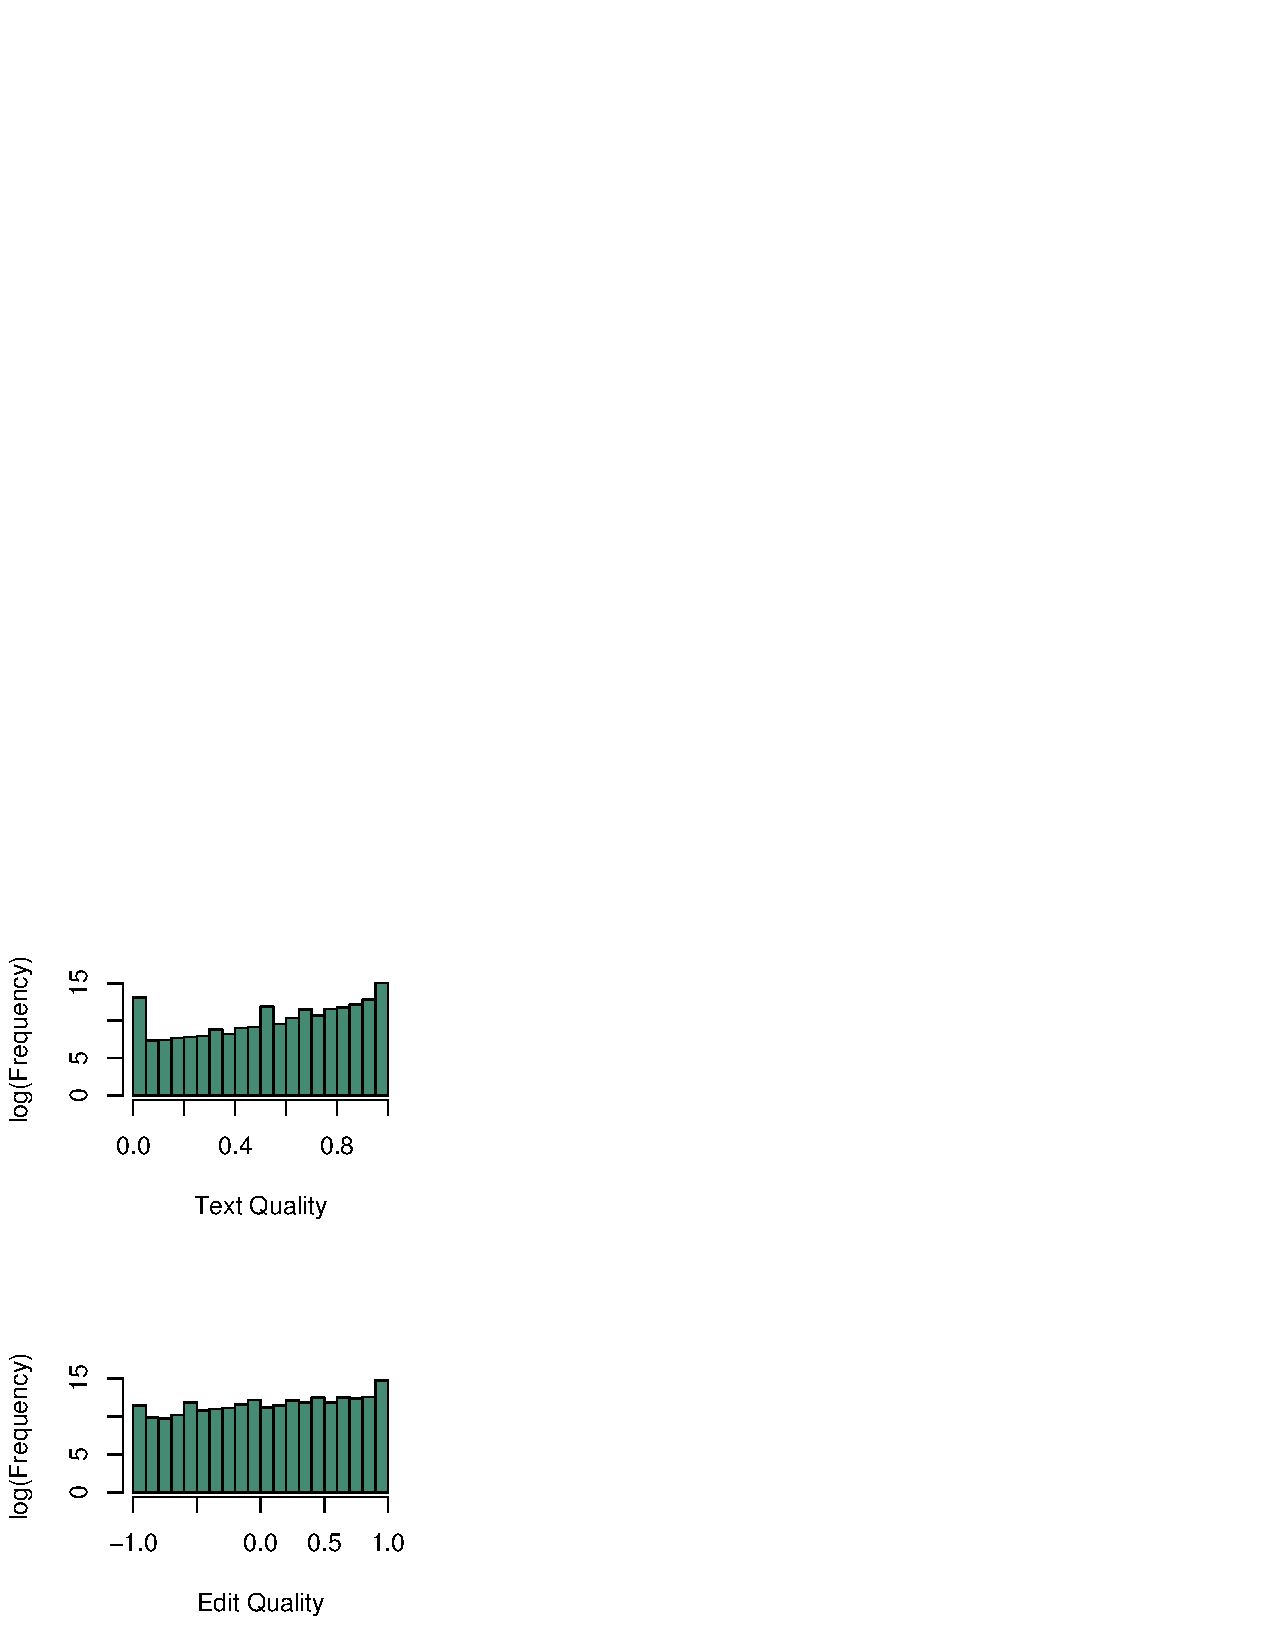
\includegraphics[width=0.70\textwidth]{part-I10-contrib/graphs/all_quality}
    }
    \end{center}
    \caption[Measuring edit and text quality over revisions]{
    	This graph shows the text quality $\quality{tdecay}{10}{}$
        and edit quality measure $\quality{elong}{10}{}$
	for 5 million randomly selected records of each type.
    }
    \label{fig-revs-quality}
\end{figure}

Delving directly into the data for text quality, we observe
that $10\%$ of the revisions made had 
$\quality{tdecay}{10}{} \le 0.05$ while $66.67\%$ of the revisions had
$\quality{tdecay}{10}{} > 0.95$.
When $\quality{tdecay}{10}{} = 0$, the text is immediately deleted
in the next revision, so we can infer that these revisions
are the work of vandals.
When we look at the size of contributions made, we noticed that
$6\%$ of the amount of new text added had $\quality{tdecay}{10}{} = 0$,
whereas $76.21\%$ of the new text added had $\quality{tdecay}{10}{} > 0.95$.
From this we conclude that authors mostly add good new text.

The data is less stark for edit quality.
When we looked at revisions, we saw that $1.9\%$ of the revisions
had $\quality{elong}{10}{} \le -0.9$, whereas $51.12\%$ had
$\quality{elong}{10}{} > 0.9$.
In fact, $84.71\%$ had positive edit quality.
In terms of edit contributions, we noticed that $7.5\%$ of the
edit contributions had $\quality{elong}{10}{} \le -0.9$, whereas
$61.39\%$ had $\quality{elong}{10}{} > 0.9$.
Moreover, $1.6\%$ of the edit contributions were immediately
reverted.
From these statistics, we conclude that authors mostly do good
edits, but that contributions are massaged a bit by later editors.

Figure~\ref{fig-revs-contrib} shows the absolute text and edit 
contributions, \txt{}{\version{i}} and \dist{}{\version{i}}, for the sets of sampled revisions.
It is important to note that these two graphs are using
the logarithm of the size of contribution, along the $x$-axis;
edit sizes can fall below $+1$, due to the way we compute
edit distance for moved words as a fraction of how much of
the document they move across.
Thus, the frequency count for edit sizes between $0$ and $1$
suggests that a good fraction of revisions involve rearranging
of text.
Beyond that, we can conclude that contributions, as measured
by text added or by edit distance, are predominantly under
100 words.
%
\begin{figure}[tbhp]
    \begin{center}
    \fbox{
    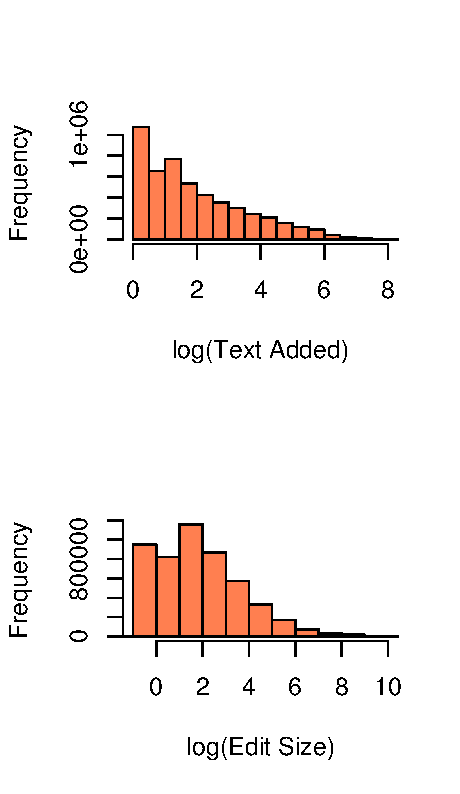
\includegraphics[width=0.70\textwidth]{part-I10-contrib/graphs/all_contrib}
    }
    \end{center}
    \caption[Measuring total edit and text contribution over revisions]{
        This graph shows the absolute text and edit contributions 
        on a log scale, for 5 million randomly selected records
	of each type.
    }
    \label{fig-revs-contrib}
\end{figure}
%

In Figure~\ref{fig-user-quality} we show the average edit quality
and average text quality for all non-anonymous authors.
In order to compute this, we took all revisions created by each 
author and took an average of the text and edit qualities of 
those revisions.
We notice that $15.9\%$ of authors had $\quality{tdecay}{10}{} \le 0.05$
and $6.3\%$ of authors had $\quality{elong}{10}{} \le -0.9$.
These are shown by the bars on the left extreme of the
histograms in Figure~\ref{fig-user-quality}.
This sharp increase in the number of authors at the lowest end
of our quality measures, combined with our previous analysis
of revisions and contributions with respect to quality, gives
us some justification to define vandals as those
authors who have either $\quality{tdecay}{10}{} \le 0.05$ or 
$\quality{elong}{10}{} \le -0.9$ on average.
We state that the identification of vandals can be made more
precise using more sophisticated analyses of our data, but we
don't deal with that in this paper.
%
\begin{figure}[tbhp]
    \begin{center}
    \fbox{
    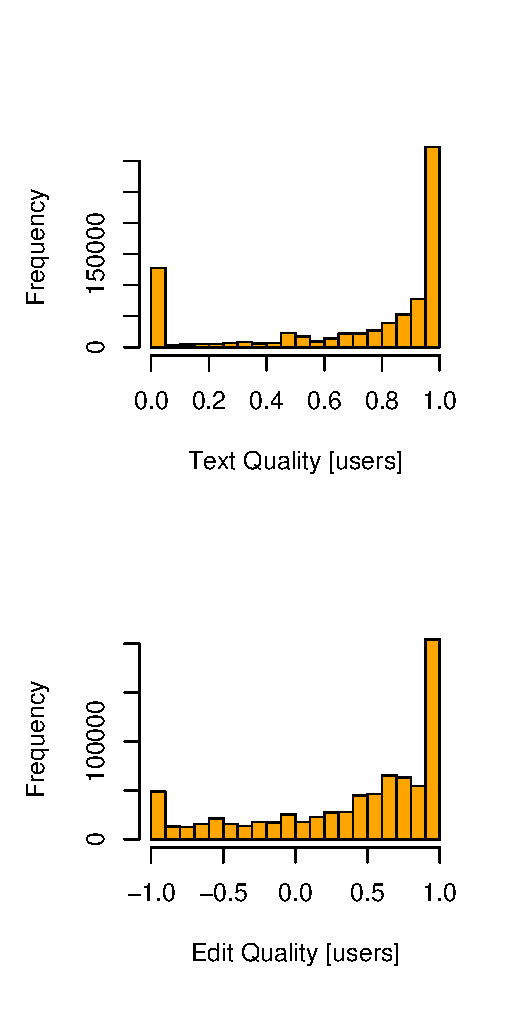
\includegraphics[width=0.60\textwidth]{part-I10-contrib/graphs/user_quality}
    }
    \end{center}
    \caption[Measuring edit and text quality for all authors]{
    	This graph shows the average text quality $\quality{tdecay}{10}{}$
	and the average edit quality measure $\quality{elong}{10}{}$
	over all non-anonymous authors.
    }
    \label{fig-user-quality}
\end{figure}
%

During our investigations comparing the proposed measures,
we found an unusually large fraction of non-anonymous authors
having scores relatively close to zero.
This suggested that many users had made a relatively
small number of revisions, and that the absolute
text and edit contributions of the revisions tended to
be small, or that the quality tended towards zero.
This is consistent with the power law distribution
for edits per author (Lotka's law) detected by~\cite{Voss2005};
we confirmed the distribution for our data (shown
in Figure~\ref{fig-hist-numedits}) and observed
that 362,461 authors made only one edit:
over 46\% of the total 777,223 authors we tracked.
In Figure~\ref{fig-singles-quality} we show the edit quality
measure for these authors.
In contrast to the edit quality distribution over
all authors from Figure~\ref{fig-revs-quality},
we notice that the edit quality for these authors
are almost evenly distributed across the
entire quality range (except for the two extreme values).
%
\begin{figure}[tbhp]
    \begin{center}
    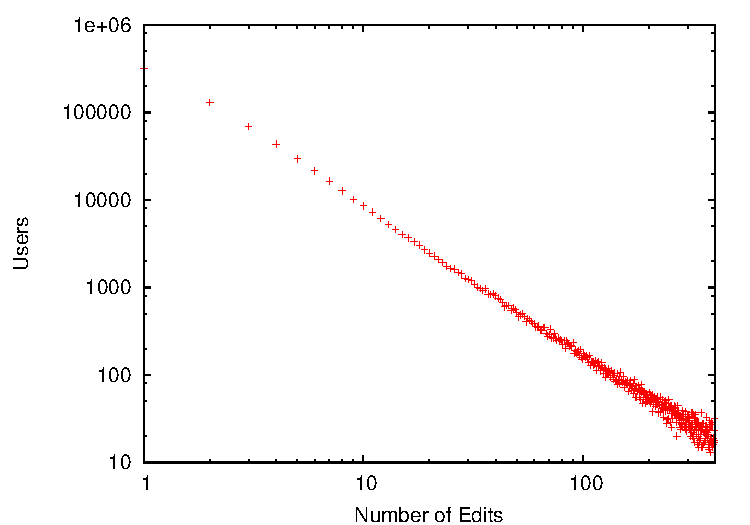
\includegraphics[width=0.75\textwidth]{part-I10-contrib/graphs/plot-hist-numedits}
    \end{center}
    \caption[Distribution of authors over number of edits]{
    	The distribution of the number of edits that each author made.
	Over 46\% of the non-anonymous authors
	make a single edit in the main English Wikipedia.
    }
    \label{fig-hist-numedits}
\end{figure}
%
\begin{figure}[tbph]
    \begin{center}
    \fbox {
    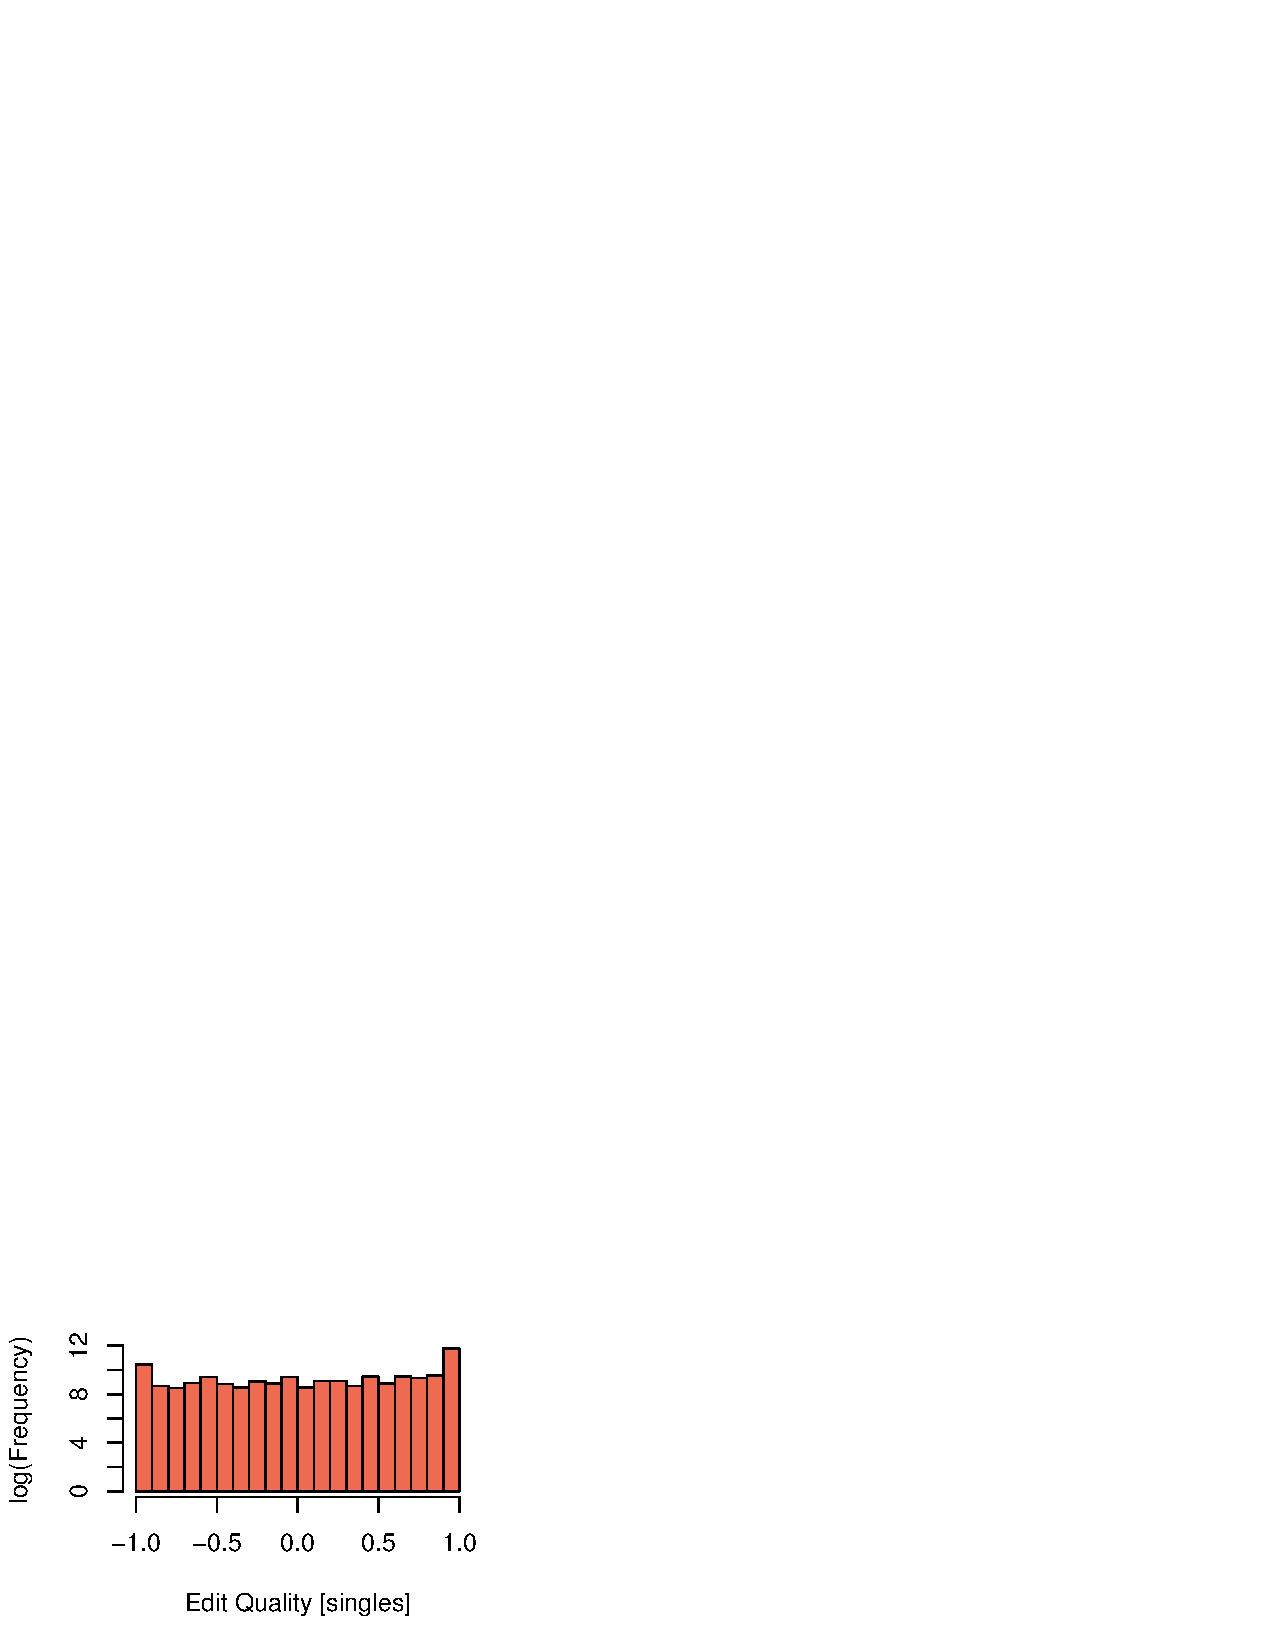
\includegraphics[width=0.70\textwidth]{part-I10-contrib/graphs/singles-quality}
    }
    \end{center}
    \caption[Edit quality of authors with one edit]{
        This plot shows the $\quality{elong}{10}{}$ of the
	non-anonymous authors who made a single edit contribution.
    }
    \label{fig-singles-quality}
\end{figure}

\pagebreak
\subsection{Comparing Measures}

We next present the correlations between the various measures
in Table~\ref{cor-tab}.
These are correlations with respect to the amount of contributions
made by all non-anonymous authors, excluding those we've classified
as vandals.  
% \mynote{Vishwa: why did we exclude vandals?  Maybe we
% should explain.  -Bo}
%
\begin{table*}[!tp]
\begin{center}
\begin{tabular}{|c||c|c|c|c|c|c|c|}
	\hline
$Measures$ &  $EditLong$ & $EditOnly$ & $NumEdits$ & $TenRevs$ & $TextLong$ & $TextOnly$ & $TextWPen$ \\
        \hline \hline
$EditLong$         &  1.000  & 0.999  &  0.28  &         0.070  & 0.075  &  0.16  & -0.32 \\
$EditOnly$         &  0.999  & 1.000  &  0.29  &         0.071  & 0.077  &  0.16  & -0.33 \\
$NumEdits$         &  0.283  & 0.286  &  1.00  &         0.361  & 0.417  &  0.45  &  0.27 \\
$TenRevs$          &  0.070  & 0.071  &  0.36  &         1.000  & 0.983  &  0.96  &  0.89 \\
$TextLong$         &  0.075  & 0.077  &  0.42  &         0.983  & 1.000  &  0.98  &  0.90 \\
$TextOnly$         &  0.158  & 0.164  &  0.45  &         0.963  & 0.983  &  1.00  &  0.82 \\
$TextWPen$         & -0.320  &-0.326  &  0.27  &         0.886  & 0.897  &  0.82  &  1.00 \\
        \hline
\end{tabular}
\end{center}
\caption[Correlations of our measures]{
This table gives the pairwise correlations of the different measures we 
have defined in this paper.
}\label{cor-tab}
\end{table*}
%
From the correlation table, we notice that text based measures are
better positively correlated with each other.
Similarly, the edit based measures are better positively correlated 
with each other as we expected.
The measures $\editlong$ and $\editonly$ are highly correlated as 
borne out by the fact that a large percentage of the edits are of
good quality.
We notice that the same is true for $\textlong$ and $\textonly$.
The correlation between $\punish$ and the absolute measure
$\editonly$ is low, demonstrating that $\punish$
penalizes authors for bad edits, gives no credit to good edits,
and accumulates the quality discounted text contribution measure 
$\textlong$.
Therefore, authors need to contribute high quality text, while
ensuring that they have no bad edits to get a high score on
$\punish$.
$\tenrevs$ being a text contribution measure, is highly correlated
with the other text contribution measures $\textonly$ and
$\textlong$.
$\numedits$ is positively correlated with all measures as we would
expect, since the majority of contributions are deemed good by
each of the quality measures.

While $\textonly$ and $\editonly$ appear to be reasonable measures 
of author contribution, we have found evidence that vandals
accrue large contributions against these measures.
For instance, we found that author $1065172$ is in the $99th$ 
percentile when measured using $\textonly$, but is nearly at the
bottom of the ranks, at $0.000001$ quantile when we look at his
$\punish$ measure.
We found five revisions in which this author added new text, but
four of those were immediately reverted.
The only revision that was kept around was a one word addition to a
page!
From the edits made by this author, we saw that he is a spammer.
On the other hand, using $\textlong$ instead of $\textonly$ we
noticed that the author was below the $25th$ percentile.
On the $\editlong$ measure, this author was below the 
$0.001$ quantile; among the lowest in rank.
Therefore, we argue that the measures that discount $\textonly$ and 
$\editonly$ by a text or edit quality measure are more indicative
of the ``useful'' work added to the Wikipedia.
We argue that $\numedits$ is not as good a measure, since 
vandals and bots can easily make large numbers of bad edits.

We present two figures, Figure~\ref{fig-zoom-editonly-editlong}
and Figure~\ref{fig-zoom-textonly-textlong},
which have been restricted to a region containing the
bulk of the data points.
In Figure~\ref{fig-zoom-editonly-editlong},
we see a vee shape, which separates the authors into
two groups: those that have positive edit quality and those
that have negative edit quality, as measured by $\avgeditquality$.
The worse the quality of edits made by authors the less they
accumulate of the $\editlong$ measure, whereas the $\editonly$
measure, being oblivious to edit quality, attributes the same
contribution to an author whose contributions persists as it 
does to an author whose contributions do not.
On the negative side of $\editlong$, there are points that represent
vandals, who edit large sections of existing pages, which are
then immediately reverted.
Clearly, $\editonly$ ranks some of these authors very highly,
whereas $\editlong$ is able to distinguish them and rank
them very low.

In Figure~\ref{fig-zoom-textonly-textlong},
we see a similar vee shape; in this case, $\textlong$
cannot go below zero as the text quality measure is always 
non-negative, so vandals, by our definition, receive no 
contribution.
As before, the measure that incorporates quality can 
distinguish vandals from non-vandals and attribute a contribution
measure to authors that is proportional to the merit of their
contribution.

Of the various measures we introduced, $\punish$ is perhaps the
one with the least tolerance, since by this measure, the only way
an author can accumulate contribution is by adding new
text that persists and by making edits that are judged to be
of good quality.
Further, this measure does not reward authors for good edits,
but penalizes them for bad edits.
In Figure~\ref{fig-zoom-textonly-textwithpunish}, we plot $\textonly$
against $\punish$.
We see the vee shape, with vandals falling on a noticeable line in
the fourth quadrant, that has no $\textonly$ contribution.
Since almost all new text added by vandals is immediate reverted,
and their edits always have low quality, we notice that they get
low negative $\punish$ contributions.
In fact, we noticed that the bottom ten authors by rank when
measured according to $\punish$ were all vandals with the exception
of $AntiVandalBot$.
We explain this in the subsection on bots.

\begin{figure}[t]
    \begin{center}
    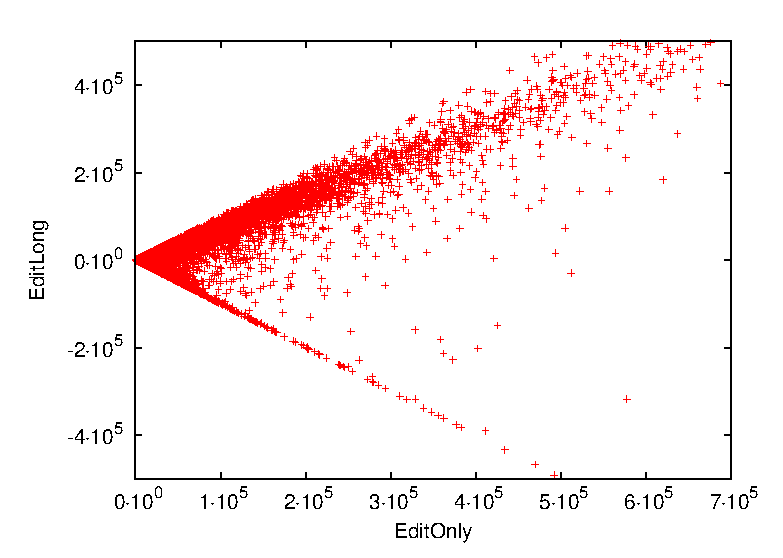
\includegraphics[width=0.45\textwidth]{part-I10-contrib/graphs/score-zoom-editonly-editlong}
    \end{center}
    \caption[EditOnly vs EditLong]{
    	Comparing the absolute edit contribution of a user
	with the edit longevity.
	Notice that authors who are ``all bad''
	are easily identifiable -- and sometimes quite prolific.
    }
    \label{fig-zoom-editonly-editlong}
\end{figure}
%
\begin{figure}[t]
    \begin{center}
    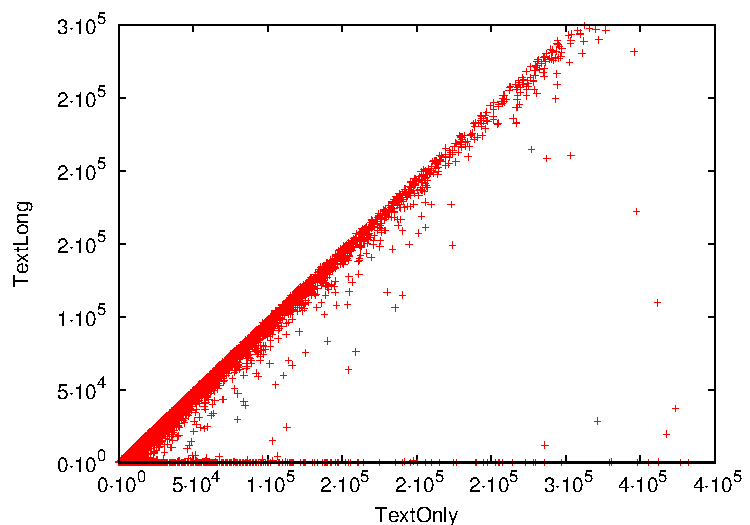
\includegraphics[width=0.45\textwidth]{part-I10-contrib/graphs/score-zoom-textonly-textlong}
    \end{center}
    \caption[TextOnly vs TextLong]{
    	Comparing the absolute text contribution with the contribution
	as measured by text longevity.
	We see that large contributors are either ``all bad''
	or nearly ``all good.''
    }
    \label{fig-zoom-textonly-textlong}
\end{figure}
%
\begin{figure}[t]
    \begin{center}
    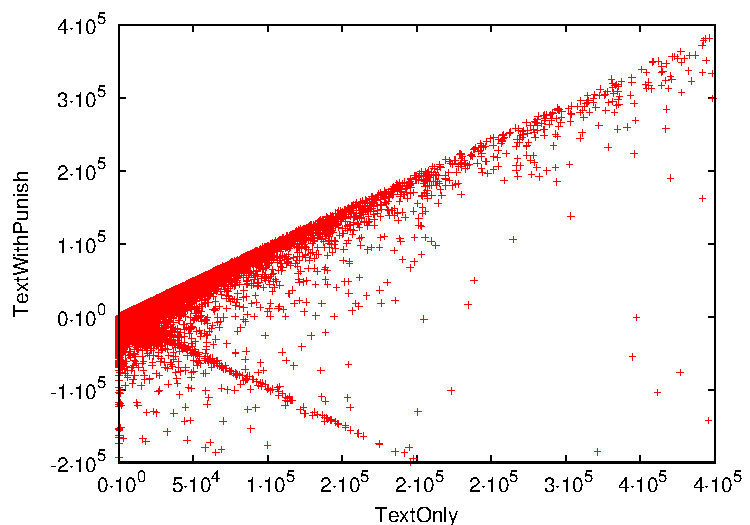
\includegraphics[width=0.45\textwidth]{part-I10-contrib/graphs/score-zoom-textonly-textwithpunish}
    \end{center}
    \caption[TextOnly vs TextWithPunish]{
    	Comparing the absolute text contribution of an author with
	their contribution as measured by \punish.
    }
    \label{fig-zoom-textonly-textwithpunish}
\end{figure}
%
\begin{figure}[t]
    \begin{center}
    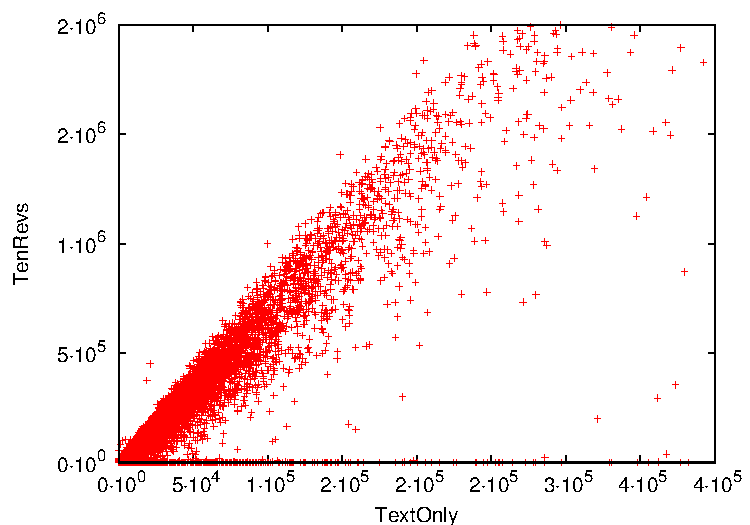
\includegraphics[width=0.45\textwidth]{part-I10-contrib/graphs/score-zoom-revisions-textonly}
    \end{center}
    \caption[Measuring short term text survival]{
    	This graph compares how much text is initially added
	by a user (along the $x$-axis), with how much
	of the text survives over the next ten filtered revisions
	(along the $y$-axis).
	The higher up the $y$-axis a point is, the more
	text that survived all ten revisions.
	Most authors add under 100,000 words,
	and about half of what they add survives.
    }
    \label{fig-zoom-revisions-textonly}
\end{figure}

\subsection{Ranking Authors}

A different direction we explored was how these different
measures end up ranking different authors.
Since the contribution measures varied over such a
wide range of values, with most people within
a smaller region around zero, we hoped that
ranking the authors would give us better insight into how
the measures differed.

To this end,  we computed the percentile rank
(rounded up to the next even value for clarity in the image)
of all non-anonymous authors, including those
that we had classified as vandals, and then plotted
them in 3-dimensional histograms; see
Figures~\ref{fig-prct-editlong-textlong}
and~\ref{fig-prct-editlong-textwithpunish}.
An important point to remember about
Figures~\ref{fig-prct-editlong-textlong}
and~\ref{fig-prct-editlong-textwithpunish}
is that the low-lying regions of the graph are
rarely zero --- there are roughly between one and ten
authors at each intersection, but this is so small compared
to the areas that correlate that we cannot see it on the graph.
Both figures show a high degree of correlation that wasn't evident
from the correlation scores in Table~\ref{tab:measure-correlations}.
Figure~\ref{fig-prct-editlong-textlong} shows that \textlong and
\editlong generally agree in the ranking of users, except for the lowest
scorers of \textlong.
The lowest scorers of \textlong all receive a score of zero, but the
``fence'' seen in the figure is an indication of the fact that there are
an enormous number of users which \textlong ranks equivalently but
\editlong is able to further distinguish between.
By contract, Figure~\ref{fig-prct-editlong-textwithpunish} shows that
\punish roughly agrees with \editlong for all users except for a thin
branch that score zero under \punish but get a positive score under
\editlong.
This thin branch represents the group of users which do not add text,
but instead only rearrange it or delete vandalism.
%
\begin{figure}[tbhp]
    \begin{center}
    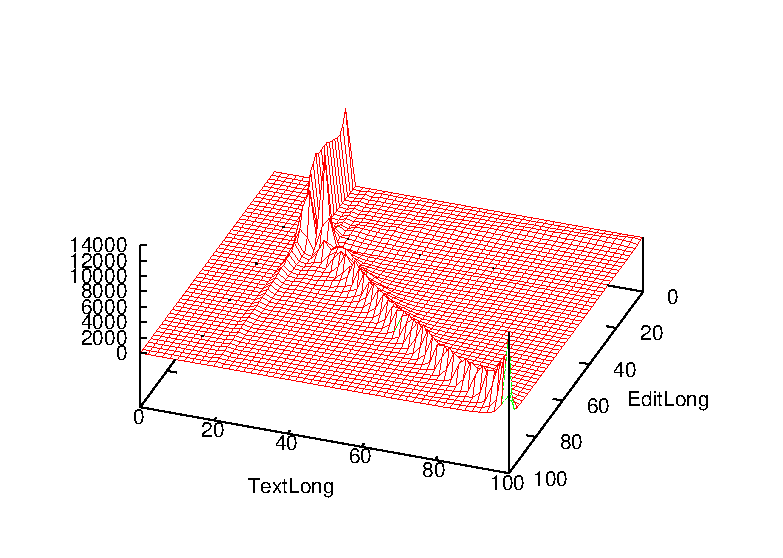
\includegraphics[width=0.85\textwidth]{part-I10-contrib/graphs/prct-editlong-textlong}
    \end{center}
    \caption[Comparing edit longevity with text longevity]{
    	$\editlong$ vs $\textlong$
    }
    \label{fig-prct-editlong-textlong}
\end{figure}
%
\begin{figure}[tbhp]
    \begin{center}
    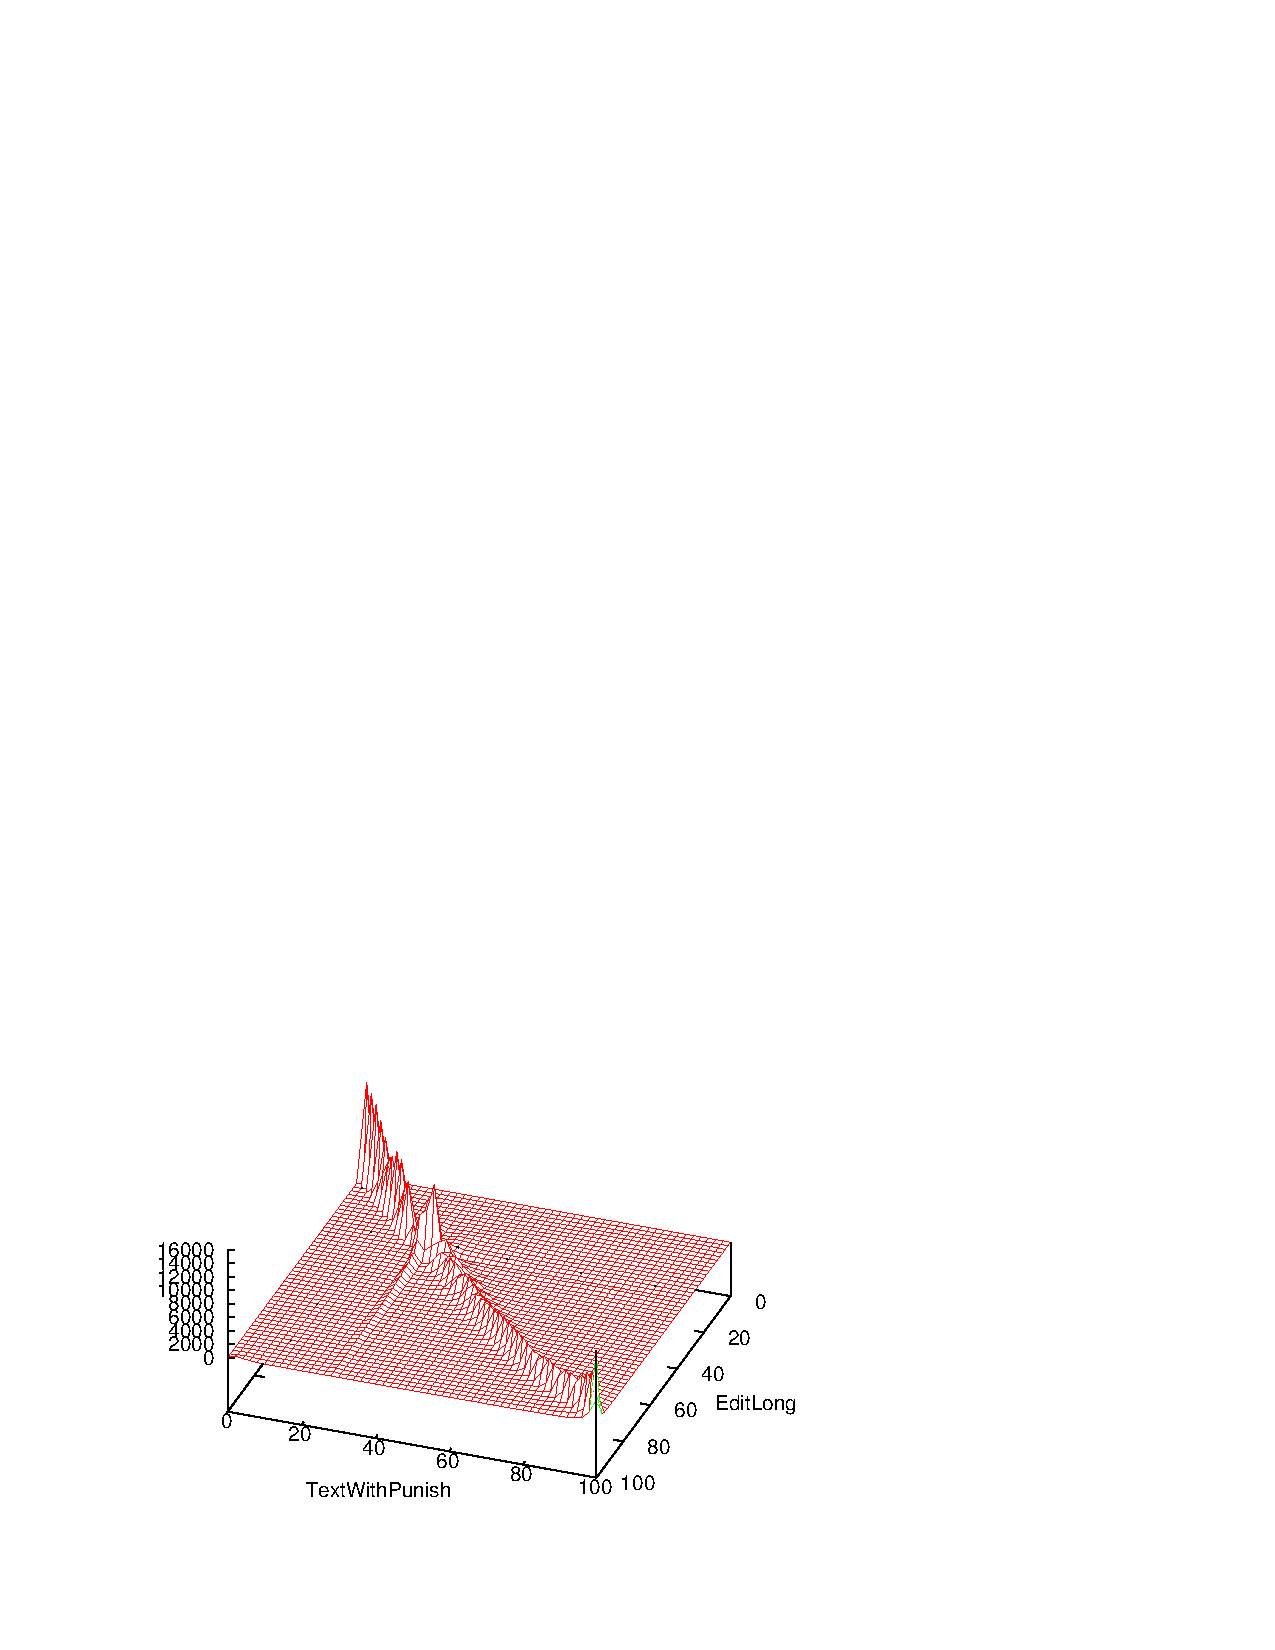
\includegraphics[width=0.85\textwidth]{part-I10-contrib/graphs/prct-editlong-textwithpunish}
    \end{center}
    \caption[Comparing edit longevity with the punishing function]{
    	$\editlong$ vs $\punish$
    }
    \label{fig-prct-editlong-textwithpunish}
\end{figure}
%

We also include a 3-dimensional histogram comparing the
percentile rankings as determined by \editlong and \numedits,
in Figure~\ref{fig-prct-editlong-numedits}.
The ``rows of fences'' we see
in Figure~\ref{fig-prct-editlong-numedits}
are due to the large number of authors who
make only a handful of edits; the \numedits measure
neither distinguishes them from each other,
nor is it capable of distinguishing good contributions from
bad contributions.
This last point is important, that even users in
the lowest percentile of \editlong can be rated
very highly by \numedits --- demonstrating
that it is much easier to game the \numedits
measure to achieve a high rank, while doing bad work.
%
\begin{comment}
%
\begin{figure}[tbhp]
    \begin{center}
    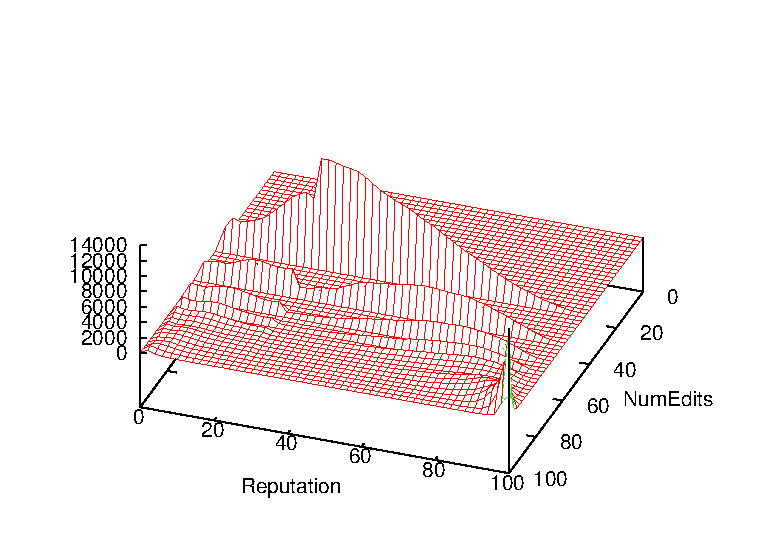
\includegraphics[width=0.85\textwidth]{part-I10-contrib/graphs/prct-numedits-reputation}
    \end{center}
    \caption[Comparing the number of edits made with the reputation function]{
    	The \contribrep measure had the highest correlation to \numedits,
	in Table~\ref{tab:measure-correlations}.
	Notice that \numedits does not distinguish well
	between users.
    }
    \label{fig-prct-numedits-reputation}
\end{figure}

\begin{figure}[tbph]
    \begin{center}
    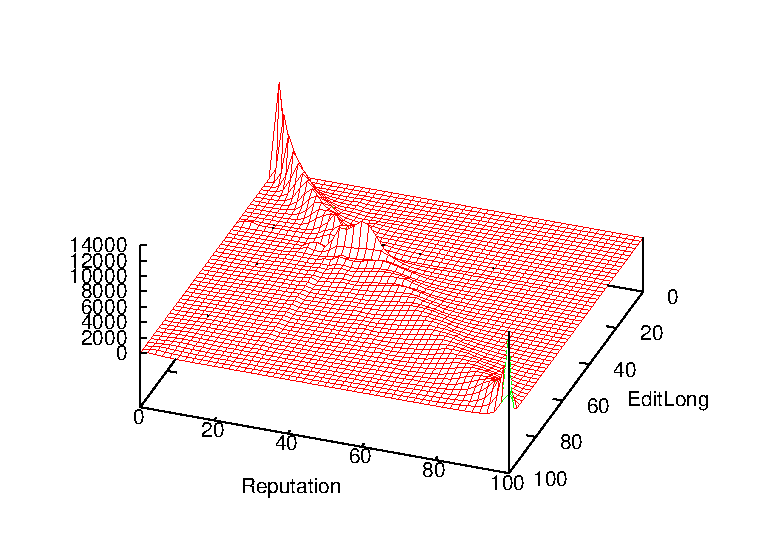
\includegraphics[width=0.85\textwidth]{part-I10-contrib/graphs/prct-editlong-reputation}
    \end{center}
    \caption[Comparing edit longevity with reputation]{
    	\editlong vs \contribrep
    }
    \label{fig-prct-editlong-reputation}
\end{figure}
%
\end{comment}

\begin{figure}[tbph]
    \begin{center}
    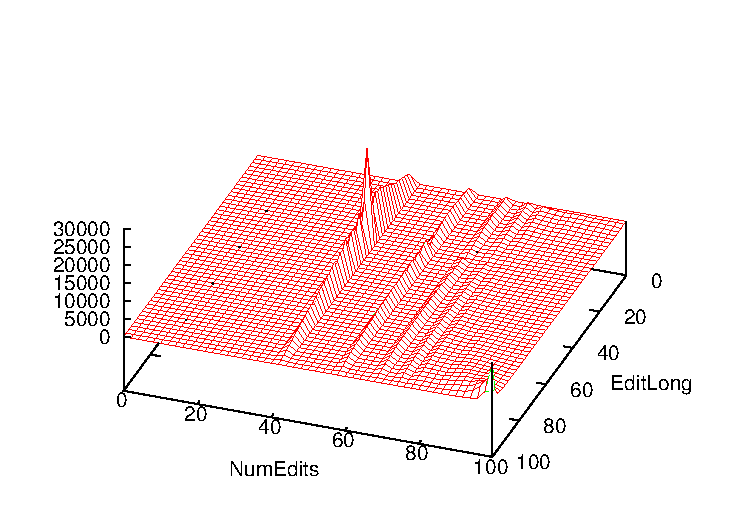
\includegraphics[width=0.85\textwidth]{part-I10-contrib/graphs/prct-editlong-numedits}
    \end{center}
    \caption[Comparing edit longevity with the number of edits made]{
    	$\editlong$ vs $\numedits$
    }
    \label{fig-prct-editlong-numedits}
\end{figure}


\subsection{Bot Behavior}

There are several bots operating on the contents of the Wikipedia.
Many bots are sanctioned by the community, and do useful
chores such as automatically removing text which is likely
to be vandalism, correcting spelling, and adding geographical data.
There are also bots which are created to vandalize pages,
and sometimes well-intentioned bots run amock and
accidentally vandalize pages as well.
During the course of comparing the various contribution
measures with each other, we found several bots (both
good and bad) which were obvious outliers in the data.
To analyze bots as a group, we selected all users
which included the ``Bot'' moniker in their username;
this self-identification does include some malicious bots,
but obviously favors selection of good bots.

The edit and text quality measures for all bots are similar to
that of all authors shown in Figure~\ref{fig-revs-quality}.
We noticed that bots create a large number of revisions with
high quality.
We found that $69.56\%$ of the revisions made by
bots have a text quality measure of $\textquality > 0.95$.
The percentage of revisions made by bots with 
$\textquality \le 0.05$ was $9.2\%$.
We found that $66.92\%$ of the new text added by bots were with
$\textquality > 0.95$ and $14.14\%$ of the new text added by
bots were with $\textquality = 0$, which means they were 
immediately reverted.
Similarly, on the edit contributions of bots we found that
$54.42\%$ of the revisions with edits made by bots were of
high edit quality, with $\avgeditquality > 0.9$.
The number of revisions having $\avgeditquality < -0.9$ being
negligible; $1\%$ from our analysis.
When we counted all edit revisions that had a negative edit
quality we saw that $12.73\%$ of the revisions were judged to 
be of poor quality with $\avgeditquality < 0$.
We found that $93.3\%$ of the edit contributions made by bots
had positive edit quality and the remaining $6.4\%$ had
negative edit quality.
More interestingly, $65.20\%$ of the edit contributions made
by bots had $\avgeditquality > 0.9$, which means they were
not edited out in subsequent revisions and represent the
sheer amount of work done by bots that is of very high quality.
The contributions with $\avgeditquality < -0.9$ are $1.8\%$.
This indicates that a large part of the text additions made by bots 
and a large part of the edit contributions made by bots survive
indefinitely.

Furthermore, our analysis indicates that bots make large amounts of
edit contributions compared to text contributions; the ratio
of the size of edits $\editonly$ to the size of new text $\textonly$
for all bots is $11.61$.
Since the penalizing measure $\punish$ does not credit authors for
good edits but reduces their $\textlong$ contributions, by the 
amount of their bad edits as measured by $\editlong$, we notice that 
edits judged as being of poor quality overwhelm the smaller text 
contributions of bots in general, and $AntiVandalBot$ in particular, 
resulting in a small overall contribution.
We also note here that $SmackBot$ did much better on this
measure.
$SmackBot$ contributes more text than $AntiVandalBot$.
Most of its edits are of smaller size than $AntiVandalBot$.
Since they have similar quality measures, $AntiVandalBot$ ends
up with a lower score on $\punish$ when compared to $SmackBot$.

\begin{comment}
%
\begin{figure*}
    \begin{center}
    \fbox{
    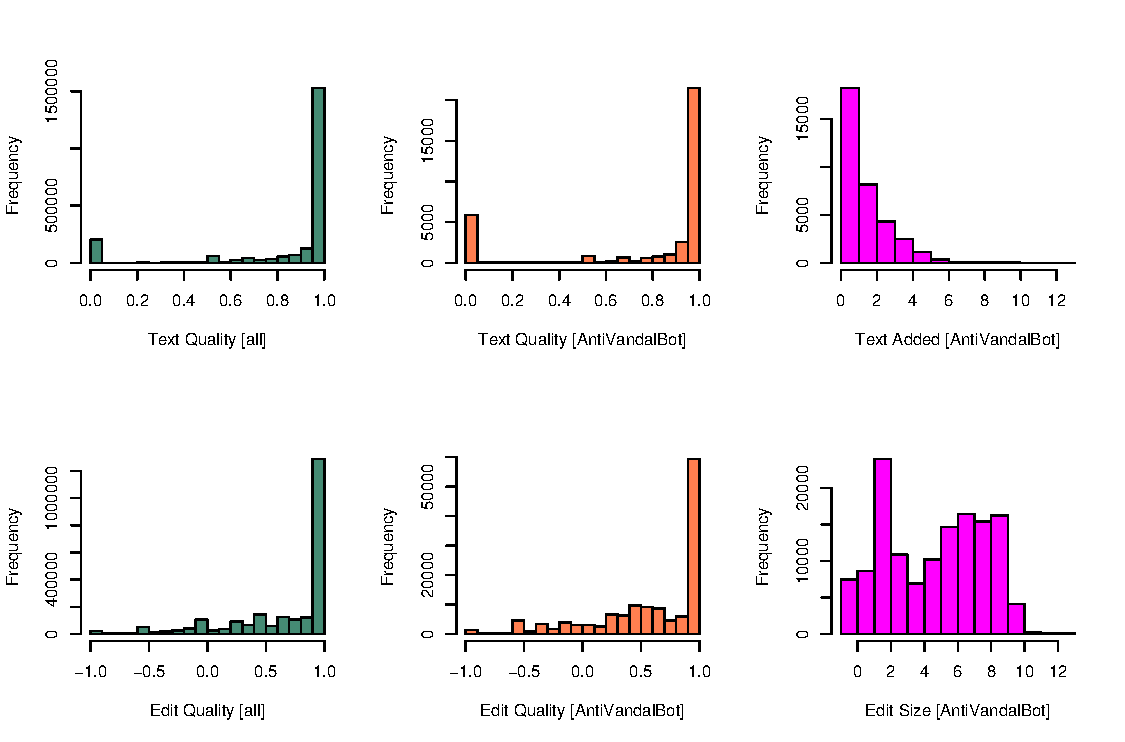
\includegraphics[scale=0.75]{part-I10-contrib/graphs/allbots_anti_hist}
    }
    \end{center}
    \caption[Measuring edit and text quality for all bots and $AntiVandalBot$]{
    	This graph shows the edit quality measure $\avgeditquality$
        and text quality $\textquality$ for all bots.
        A quality measure of $1$ indicates that all the changes
        were preserved.
        A quality measure of $0$ indicates that all the changes
        were reverted in the very next revision.
        The histograms on the left are for all bots.
        The ones on the right are the quality measures and the absolute amounts
        of text and edit contributions for $AntiVandalBot$.
    }
    \label{bot-contribs}
\end{figure*}
\end{comment}

\subsection{Sources of Error}

Since we use filtered revisions, namely we collapse all consecutive
revisions by the same author, and since we treat all anonymous authors
identically, consecutive edits made by anonymous authors cannot be
distinguished.
We therefore discard all anonymous authors from our analysis: in any
case, we are not measuring their contributions, as they cannot be
individually attributed. 
We have noticed that there are anonymous authors who do good work
on the Wikipedia, but at this point we have not implemented a
mechanism to attribute them a contribution measure.

We ignore the time difference between edits.
When pages receive many views with little editing, it suggests 
that the article is substantially correct;
perhaps later edits are due to changing facts, and not because 
of poor quality.
Articles which are the subject of current events are 
particularly likely to have their edit quality misjudged.
Relatedly, grouping revisions by author ignores the fact that 
edits separated by days or months are less related and have most 
likely been reviewed by others.




\subsection{Comparing Contributions}

Defining multiple contribution measures affords us
the opportunity to examine and quantify the
user behaviors over the large scale of edits performed.
We looked at the list of all blocked authors.~\footnote{Retrieved
on May 8, 2008, directly from the Wikipedia database.
It corresponds to the data available at
\url{http://en.wikipedia.org/wiki/Wikipedia:List_of_banned_users}.}
We separated them from the others with the objective of determining 
how many of these authors met our definition of vandals.
We were surprised to note that over $51\%$ of authors had 
$\quality{tdecay}{10}{} > 0.95$ and $39\%$ of authors had 
$\quality{elong}{10}{} > 0.9$.
In fact, over $47\%$ of the blocked authors make text contributions 
that have an average text quality over $0.95$.
Similarly, over $32\%$ of the these authors make edit contributions
that have an average edit quality over $0.9$.
We note that $11.2\%$ of these authors qualify as vandals by our measure,
based on their average edit quality and $24.9\%$ qualify as vandals
based on their average text quality.
But a large percentage of the authors in the blocked authors 
list are not vandals, as determined by our definition.

A couple of cases in point are those of authors $3362$ and 
$10784$.
They are both blocked, but are over the $99th$ percentile on 
\editlong, \textlong and \punish.
One was blocked by Jimbo Wales and the other was blocked as he
was suspected of using multiple accounts.

We end this subsection, by mentioning the top rankers against all
measures.
The highest ranks across all contributions were secured by
authors $3903$ and \textit{AntiVandalBot}.
Author $3903$ had the top rank with respect to measures
\textonly, \textlong, \punish and \tenrevs.
\textit{AntiVandalBot} had the top rank with respect to the measures
\editlong and \editonly.
Interestingly, \textit{SmackBot} was the second highest scorer after
author $3903$ on measures \textlong and \punish.


\section{Conclusions}

We propose two measures of revision quality computed
from Wikipedia's revision history.
The measure \textit{text longevity} is based on an intuitive
model of computing the text added by authors at each revision
and detecting how much of that text remains within the article
in subsequent revisions; to account for the variation in
the amount of preserved text over the subsequent revisions,
we model the change as a geometrically decaying process
and compute the decay rate as a single value to describe
the variation.
The measure \textit{edit longevity} was developed to address
the reality that authors also delete and rearrange text,
and that these are valuable contributions to the Wikipedia.
We use edit distance~\cite{Levenshtein1966} to describe the
amount of \intro{effort} that an author puts into making a
revision to an article; this is the basis for computing
edit longevity, which estimates the amount of effort by an
author that brings the article text closer to some future
version of the article.

We evaluate these two measures using the PAN-WVC-10 dataset, which is
manually annotated to indicate which revisions are vandalism and which
are well-intentioned edits, and treat each as a predictor of vandalism.
We find that edit longevity performs much better than text longevity,
but even text longevity does better than chance at predicting vandalism.
Overall, these results are encouraging for using edit longevity and text
longevity as signals for inferring the community feedback of an author's
edit.  Knowing the quality of edits, we can build an author reputation
system upon these signals; we describe such a system in
Chapter~\ref{ch:reputation}.



% \bibliographystyle{plain}
% \bibliography{dvlab}

\begin{thebibliography}{10}

\bibitem{trust-techrep-07}
B.T. Adler, J.~Benterou, K.~Chatterjee, L.~de~Alfaro, I.~Pye, and V.~Raman.
\newblock Assigning trust to wikipedia content.
\newblock Technical Report UCSC-CRL-07-09, School of Engineering, University of
  California, Santa Cruz, CA, USA, 2007.

\bibitem{www07}
B.T. Adler and L.~de~Alfaro.
\newblock A content-driven reputation system for the {Wikipedia}.
\newblock In {\em Proc. of the 16th Intl. World Wide Web Conf. (WWW 2007)}.
  {ACM} Press, 2007.

\bibitem{AdministratorMop2008}
M.~Burke and R.~Kraut.
\newblock Taking up the mop: identifying future {W}ikipedia administrators.
\newblock In {\em CHI '08: CHI '08 extended abstracts on Human factors in
  computing systems}, pages 3441--3446, New York, NY, USA, 2008. ACM.

\bibitem{EditDistanceMoves}
G.~Cormode and S.~Muthukrishnan.
\newblock The string edit distance matching problem with moves.
\newblock {\em ACM Trans. Algorithms}, 3(1):2, 2007.

\bibitem{Wikis01}
W.~Cunningham and B.~Leuf.
\newblock {\em The Wiki Way. {Quick} Collaboration on the Web}.
\newblock Addison-Wesley, 2001.

\bibitem{SLOC1992}
R.~E.~Park et~al.
\newblock Software size measurement: A framework for counting source
  statements.
\newblock Technical Report CMU/SEI-92-TR-020, Carnegie Mellon University,
  September 1992.

\bibitem{AckCounting2004}
C.~L. Giles and I.~G. Councill.
\newblock Who gets acknowledged: Measuring scientific contributions through
  automatic acknowledgement indexing.
\newblock {\em Proc. of the National Academy of Sciences}, 101(51):17599 --
  17604, 2004.

\bibitem{Bourgeoisie2007}
A.~Kittur, E.~Chi, B.~A. Pendleton, B.~Suh, and T.~Mytkowicz.
\newblock Power of the {F}ew vs. {W}isdom of the {C}rowd: {W}ikipedia and the
  rise of the {B}ourgeoisie.
\newblock {\em Alt.CHI}, 2007.

\bibitem{KPB2006}
N.~Korfiatis, M.~Poulos, and G.~Bokos.
\newblock Evaluating authoritative source using social networks: an insight
  from {W}ikipedia.
\newblock {\em Online Information Review}, 30(3):252--262, 2006.

\bibitem{Levenshtein66}
V.I. Levenshtein.
\newblock Binary codes capable of correcting insertions and reversals.
\newblock {\em Sov.\ Phys.\ Dokl.}, 10:707--710, 1966.

\bibitem{WikiMTWtrust06}
D.L. McGuinness, H.~Zeng, P.P. da~Silva, L.~Ding, D.~Narayanan, and M.~Bhaowal.
\newblock Investigation into trust for collaborative information repositories:
  {A} {Wikipedia} case study.
\newblock In {\em Proceedings of the Workshop on Models of Trust for the Web},
  2006.

\bibitem{OrtegaBarahona2007}
F.~Ortega and J.~M.~G. Barahona.
\newblock Quantitative analysis of the {W}ikipedia community of users.
\newblock In {\em WikiSym '07: Proceedings of the 2007 international symposium
  on Wikis}, pages 75--86, New York, NY, USA, 2007. ACM.

\bibitem{PageRank98}
L.~Page, S.~Brin, R.~Motwani, and T.~Winograd.
\newblock The {PageRank} citation ranking: Bringing order to the web.
\newblock Technical report, Stanford Digital Library Technologies Project,
  1998.

\bibitem{R2007}
{R Development Core Team}.
\newblock {\em R: A Language and Environment for Statistical Computing}.
\newblock R Foundation for Statistical Computing, Vienna, Austria, 2007.
\newblock {ISBN} 3-900051-07-0.

\bibitem{MITRE1988}
H.~P. Schultz.
\newblock Software management metrics.
\newblock Technical Report AD-A196 916, MITRE, May 1988.

\bibitem{CognitiveSurplus2008}
C.~Shirky.
\newblock Gin, television, and social surplus.
\newblock
  \url{http://www.herecomeseverybody.org/2008/04/looking-for-the-mouse.html},
  April 2008.
\newblock (Retrieved on 9-May-2008.).

\bibitem{SteinHess2007}
K.~Stein and C.~Hess.
\newblock Does it matter who contributes: a study on featured articles in the
  german wikipedia.
\newblock In {\em HT '07: Proceedings of the 18th conference on Hypertext and
  hypermedia}, pages 171--174, New York, NY, USA, 2007. ACM.

\bibitem{WikiDashboard2008}
B.~Suh, E.~H. Chi, A.~Kittur, and B.~A. Pendleton.
\newblock Lifting the veil: improving accountability and social transparency in
  {W}ikipedia with wikidashboard.
\newblock In {\em CHI '08: Proceeding of the twenty-sixth annual SIGCHI
  conference on Human factors in computing systems}, pages 1037--1040, New
  York, NY, USA, 2008. ACM.

\bibitem{Swartz2006}
A.~Swartz.
\newblock Who writes {W}ikipedia?
\newblock \url{http://www.aaronsw.com/weblog/whowriteswikipedia}, September
  2006.
\newblock (Retrieved on 9-May-2008.).

\bibitem{TichyEditDist}
W.F. Tichy.
\newblock The string-to-string correction problem with block move.
\newblock {\em {ACM} Trans.\ on Computer Systems}, 2(4), 1984.

\bibitem{Voss2005}
J.~Vo\ss{}.
\newblock Measuring wikipedia.
\newblock In {\em Proc.\ of the 10th Intl.\ Conf.\ of the ISSI}, 2005.

\bibitem{EditDist74}
Robert~A. Wagner and Michael~J. Fischer.
\newblock The string-to-string correction problem.
\newblock {\em J. ACM}, 21(1):168--173, 1974.

\bibitem{Wales2005}
J.~Wales.
\newblock Wikipedia, emergence, and the wisdom of crowds.
\newblock
  \url{http://lists.wikimedia.org/pipermail/wikipedia-l/2005-May/021764.html},
  May 2005.
\newblock (Retrieved 9-May-2008.).

\bibitem{EditsEqQuality2007}
D.~M. Wilkinson and B.~A. Huberman.
\newblock Cooperation and quality in wikipedia.
\newblock In {\em WikiSym '07: Proceedings of the 2007 international symposium
  on Wikis}, pages 157--164, New York, NY, USA, 2007. ACM.

\end{thebibliography}

\end{document}
